% https://tex.stackexchange.com/questions/367315/tikz-feynman-too-big-vertex-label
\documentclass[tikz, border=10pt]{standalone}
\usepackage{siunitx}
\usepackage{physics}
\usetikzlibrary{shapes}
\usetikzlibrary{arrows,decorations.markings,calc,fadings,decorations.pathreplacing, patterns, decorations.pathmorphing, positioning}

\newcommand{\AxisRotator}[1][rotate=0]{%
    \tikz \draw[color=red, x=.5em,y=1.25em,line width=.15ex,-stealth,#1] (0,0) arc (-150:150:1 and 1);%
}

\begin{document}
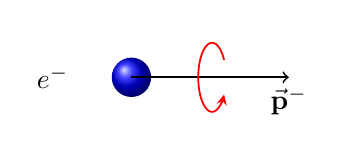
\begin{tikzpicture}
	\node[circle,shading=ball,minimum width=0.5cm] (ball) at (0,0) {};
	\draw [line width=.15ex,->] (0,0) -- (2,0);
	\draw (1,0) node {\AxisRotator[rotate=-180]};
	\draw (-1,0) node {\( e^- \)};
	\draw (2,0) node[below] {\( \va{p}^- \)};
\end{tikzpicture}
\end{document}
